\documentclass{report}

\usepackage[utf8]{inputenc}
\usepackage[T1]{fontenc}
\usepackage{mathtools}
\usepackage[thinc]{esdiff}
\usepackage{amsmath}
\usepackage{graphicx}
\usepackage{stackengine}
\stackMath


\begin{document}
	\setcounter{chapter}{2}
	\chapter{Common families of Distribution}
		
\section{}
EX = {$\frac{1}{N_{1} - N_{0} + 1}($$\sum_{x=0}^{N_{1}}i - \sum_{x=0}^{N_{0} - 1}i) = \frac{N_{1} + N_{0}}{2}$}
\newline
EX{\textsuperscript{2}} = {$\frac{1}{N_{1} - N_{0} + 1}(\frac{(N_{1})(N_{1} + 1)(2N_{1} + 1) - (N_{0} - 1)(N_{0})(2N_{0} - 1)}{6})$}
\newline
Var = {$\frac{(N_{1} - N_{0})(N_1 - N_0 + 2)}{12}$}
\newline

\section{}
(a) P(X = 0 {$\vert$} M = 100,N = 6,K) = $\frac{\left(\stackanchor{6}{0}\right) \left(\stackanchor{94}{K}\right)}{\left(\stackanchor{100}{K}\right)}$
On solving K=32
{\newline}
(b) P(X = 0 {$\vert$} M = 100,N = 6,K) = $\frac{\left(\stackanchor{6}{0}\right) \left(\stackanchor{94}{K}\right)}{\left(\stackanchor{100}{K}\right)} + \frac{\left(\stackanchor{6}{1}\right) \left(\stackanchor{94}{K-1}\right)}{\left(\stackanchor{100}{K}\right)}$
{\newline}
On solving K = 50
{\newline}

\section{}
(a) So pedestrian have to pass and that could have happen at any event of time lets say at 10 sec so past 3 secs need to be (1-p){\textsuperscript{3}}.
Now for the first 4 seconds car passes at 1{\textsuperscript{st}} second and rest none would be p(1-p){\textsuperscript{3}}We nee to do at any seconds after 4 would be (1 - p(1-p){\textsuperscript{3}})(1-p){\textsuperscript{3}}
{\newline}

\section{}
(a) So EX = {$\sum_{i=0}^{\infty}\sum_{j=0}^{\infty}i\left(\frac{n-1}{n}\right)^j\left(\frac{1}{n}\right)$} = n
\newline
(b) So EX = 
{$\sum_{i=0}^{\infty}\sum_{j=0}^{\infty}i\left(\frac{n-i}{n}\right)^j\left(\frac{1}{n}\right)$} = $\frac{n+1}{2}$
{\newline}

\section{}
(doubtful)

\section{}
(a) binomial distribution
\newline
(b) $\sum_{x=0}^{100} \quad \textsuperscript{2000}C_x\left(\frac{1}{100}\right)^x\left(\frac{99}{100}\right)^{2000-x}$
\newline
(c) $\lambda$ = 2000 * $\frac{1}{100}$ = 20
\newline
P(X=100) = $\frac{1}{e^{20}}\left[1 + \sum_{i=1}^{i=100}\frac{20^{i}}{i!}\right] = .99 \Rightarrow 99 percent$
\newline

\section{}
1 - $\frac{1}{e^\lambda}$ - $\frac{\lambda}{e^\lambda}$ = 0.99 $\Rightarrow$
$\lambda$ = 6.638
\newline

\section{}
(doubtful)

\section{}
(a) X {$\sim$} Binomial(60, $\frac{1}{90}$)
{\newline}
P(X $\ge$ 5) = 1 - $\sum_{x = 0}^{4} \left(\stackanchor{60}{2x}\right)\left[\frac{1}{90}\right]^{2x}\left[\frac{89}{90}\right]^{60 - 2x}$ Let say answer is .0006
\newline
(b) P $\sim$ Binomial(310, .0006) $\Rightarrow$ P(X $\ge$ 0) = 1 - $\left(\stackanchor{310}{0}\right) .0006^0 (1 - .0006)^{310}$ = .1698
\newline
(c) P $\sim$ Binomial(500, .1698) $\Rightarrow$ P(X $\ge$ 0) = 1 - $\left(\stackanchor{310}{0}\right) .0006^0 (1 - .0006)^{310}$ {$\sim$} 1
\newline

\section{}
(a) Hyper-geometric distributions

P = $\frac{\left(\stackanchor{N}{4}\right)\left(\stackanchor{M}{2}\right)}{\left(\stackanchor{N + M}{4}\right)\left(\stackanchor{N + M - 4}{2}\right)}$

(b) N + M = 496
\newline

$\max$ (N)(N-1)(N-2)(N-3) * (M)(M-1)
on solving N = 331, M = 496 - 331 = 
\newline

\section{}
(a) P(X = x|N, M, K) = $\frac{\left(\stackanchor{M}{x}\right)\left(\stackanchor{N - M}{K - x}\right)}{\left(\stackanchor{N}{K}\right)}$
\newline
P = $\frac{M!}{x!M-x!} * \frac{N-M!}{K-x!(N - M - (K - x))} * \frac{K!}{N!N-K!}$
P = $\left(\stackanchor{K}{x}\right)\left(\frac{M!N-M!}{N!M-x!(N-M - (K - x))}\right)$
\newline
P = $\left(\stackanchor{K}{x}\right)\left(\frac{(M * M-1 * M-2 ... M-x+1) * (N - M * N - M -1  ... N - M - (K - x))}{N * N - 1 * N - 2 ... N - k + 1}\right)$
\newline
Applying limits M $\rightarrow \infty$,M $\rightarrow \infty$ N/M M $\rightarrow$ p
\newline
Applying limits
\newline
P = $\left(\stackanchor{K}{x}\right)\left(\frac{M^{x}N^{K - x}(1 - p)^{K - x}}{N^{K}}\right)$
\newline
P = $\left(\stackanchor{K}{x}\right)p^x(1 - p)^{K - x}$
\newline
(b) See text
{\newline}
(c) Using some steps from above
\newline
P = $\left(\frac{M!N-M!K!N-K!}{x!M-x!N-M-K+x!N!}\right)$
\newline
P = $\frac{1}{x!}\left[\frac{M^xK^x}{M^x}\right]\left[1 - \frac{K}{N}\right]^{M-x}$
\newline
P = $\frac{\lambda^x}{x!}\left[1 - \frac{\lambda}{M}\right]^{M} = \frac{e^{-\lambda}\lambda^x}{x!}$
\newline

\section{}
$F_X(r - 1) = P(X \le r - 1) \newline = P($in n trial total of r{\textsuperscript{th}} success$) \newline = 1 - P($in n trail total for r\textsuperscript{th} failure$) \newline = 1 - P($in n trail total for (r+1)\textsuperscript{th} success$)$ (doubtful)

\section{}
(a) P(X{\textsubscript{T} = x}) = $\frac{P(X = x)}{P(X > 0)} \newline$
$P(X\textsubscript{T} = x) = \frac{e^{-\lambda}\lambda^x}{x!(1 - e^{-\lambda})}$
\newline
EX = $\frac{\lambda}{1 - e^{-\lambda}}$
EX{\textsuperscript{2}} = $\frac{\lambda^{2} + \lambda}{1 - e^{-\lambda}}$
\newline
VarX = $\frac{\lambda^{2} + \lambda}{1 - e^{-\lambda}}$ - $\left[\frac{\lambda}{1 - e^{-\lambda}}\right]^{2}$
\newline
(b) P(X{\textsubscript{T} = x}) = $\frac{P(X = x)}{P(X > 0)} \newline
 = \frac{\left(\stackanchor{r + y - 1}{y}\right)p^r(1 - p)^y}{1 - p^r} \newline
EX = \frac{r(1 - p)}{p(1 - p^r)}
EX = \frac{r(1 - p) - r^2(1 - p)^2}{p^2(1 - p^r)} - \left(\frac{r(1 - p)}{p(1 - p^r)}\right)^2
$
\section{}
(a) $\sum_{x=1}^{x=\infty}\frac{(1-p)^{x}}{x} =  - log(1 - (1 - p))$
So P(X = x) = 1
\newline
(b) EX = -$\frac{1}{log p} \left[\frac{1 - p}{p}\right]$
\newline
EX{\textsuperscript{2}} = -$\frac{1}{log p} \left[\frac{1 - p}{p^2}\right]$
\newline
VarX = $\frac{-(1 - p)}{p^2log p}\left[1 + \frac{1 - p}{log p}\right]$
\newline

\section{}
$M_{X}(t) = \left[\frac{p}{(1 - (1 - p)e^t)}\right]^r$
\newline
$M_{X}(t) = \left[1 + \frac{1 r(1-p)(e^t - 1)}{r (1 - (1 - p)e^t)}\right]^r$
\newline
$M_{X}(t) = \lambda(e^t - 1)$
\newline

\section{}
(a) $\Gamma(\alpha) = \int_{t=0}^{t=\infty}t^{\alpha}e^{-t}dt  = \left[t^{\alpha}e^{-t}\right]^{\infty}_{0} + \alpha\int_{t=0}^{\infty}t^{\alpha - 1}e^{-t}dt = \alpha\Gamma(\alpha)$
\newline
(b) $\left(\int_{0}^{\infty}e^{-\frac{z^2}{2}}dz\right)^2 = \left(\int_{0}^{\infty}e^{-\frac{u^2}{2}}du\right)\left(\int_{0}^{\infty}e^{-\frac{v^2}{2}}dv\right)$
\newline
$\int_{0}^{\infty} \int_{0}^{\infty}e^{\frac{-(u^2 + v^2)}{2}}dudv$ = $\frac{\sqrt{\pi}}{2}$
taking u = rcos($\theta$), v = rsin($\theta$)
\newline
$\Gamma(\frac{1}{2}) = \int_{0}^{\infty}w^{-1/2}e^{-w}dw = \sqrt{\pi}$
\newline

\section{}
$f(x|\alpha, \beta) = \frac{1}{\Gamma(\alpha)\beta^{a}}x^{\alpha - 1}e^{\frac{-x}{\beta}}$
\newline
EX = $\frac{1}{\Gamma(\alpha)\textit{$\beta$}^{\alpha}}\int_{0}^{\infty}x^{v + \alpha - 1}e^{\frac{-x}{\beta}}dx$ taking y = $\beta$x will simplify the expression.
\newline

\section{} 
$M_x(t) = \left[\frac{p}{(1 - (1 - p)e^{ty})}\right]^r$
\newline
Applying limit
\newline
$\lim_{p \rightarrow 0}\left[\frac{p}{(1 - (1 - p)e^{ty})}\right]^r$
\newline
Using L'Hospital Rule
\newline
$M_x(t) = \left[\frac{1}{-[(1-p)te^{tp} - e^{tp}]}\right]^r$
\newline
$M_x(t) = \left(\frac{1}{1 - t}\right)^r$
\newline

\section{}
On integration by parts 
\newline
$\int_{x}^{\infty}\frac{1}{\Gamma(\alpha)}z^{\alpha - 1}e^{-z} = \sum_{\alpha=\alpha}^{0}\left[\frac{x^{\alpha - 1}}{\alpha!e^{x}}\right]$
\newline
On rearranging the terms
\newline
$\sum_{y=0}^{\alpha - 1}\left[\frac{x^{y}}{y!e^{x}}\right]$
\newline

\section{}
(a) EX = $\sqrt{\frac{\pi}{2}}$, EX\textsuperscript{2} = 1
\newline
(b) $f_y(y) = \frac{1}{\Gamma(\alpha)\beta^\alpha}y^{\alpha - 1}e^{\frac{-y}{\beta}}$
\newline
Y = g(X) $\Rightarrow$ X = $g^{-1}(Y)$
\newline
$f_y(y) = f_x(g^{-1}(Y))\left|\frac{dg^{-1}(Y)}{dx}\right|$
\newline
$f_y(y) = \frac{2}{\sqrt{2\pi}}e^{\frac-{g^{-1}(x)^2}{2}}\left|\frac{dg^{-1}(Y)}{dx}\right|$
let $g^{-1}(x)^2 = y$
so $\beta$ = 2
on solving $\alpha$ = -$\frac{1}{2}$
\newline

\section{}
Integral is infinite
f(x) = $\int_{-\infty}^{\infty}\frac{1}{\pi} * \frac{1}{1 + x^2} * e^{tx}dx$
\newline

\section{}
(a), (b), (c), (d), (e) Integration and parts, Do rough work
\newline

\section{}
(a) $\int_{x = \alpha}^{\infty}\frac{\beta\alpha^{\beta}}{x^{\beta + 1}}dx = -\left[\frac{\beta\alpha^{\beta}}{\beta x^{\beta}}\right]^{\infty}_{\alpha}$ = 1
\newline
(b)EX = $\int_{x = \alpha}^{\infty}x\frac{\beta\alpha^{\beta}}{x^{\beta + 1}}dx = \frac{\alpha\beta}{1 - \beta}$
\newline
EX{\textsuperscript{2}} = $\int_{x = \alpha}^{\infty}x^2\frac{\beta\alpha^{\beta}}{x^{\beta + 1}}dx = \frac{\alpha\beta}{1 - \beta} = \frac{\alpha\beta^{2}}{2 - \beta}$
\newline
Var = $\frac{\alpha\beta^{2}}{2 - \beta}$ - $\left[\frac{\alpha\beta}{1 - \beta}\right]^{2}$
\newline
(c) If $\beta$ < 2 the var is infinite
\newline

\section{}
$h_{T}(t) = \lim_{\delta \rightarrow 0}\frac{P(t \le T < t + \delta)}{P(T \ge t)}$
\newline
As $\delta$ $\rightarrow$ 0, t $\rightarrow$ T
\newline
$h_T(t) = \frac{f_T(t)}{1 - F_T(t)}$
\newline

\section{}
(a), (b), (c) simple calculation
\newline

\section{}
differentiate the function and solve it for zero

\section{}
for (a), (b), (c), (d) Equate with all the function and get the desired result.
$f(x \vert \theta) = h(x)c(\theta)exp\left(\sum_{i=1}^{k} w_{i}(\theta)t_i(x)\right)$
Equate term by term
\newline 

\section{}
Equate terms and get the result!
\newline

\section{}
(a) $f(x \vert \mu, \sigma^2) = \frac{1}{\sqrt{2\pi}\sigma}e^{\left(-\frac{(x - \mu)^2}{2\sigma^2}\right)}$
\newline
h(x) = 1 for all x;
\newline
c($\theta$) = c($\mu$, $\sigma$) = $\frac{1}{\sqrt{2\pi}\sigma}e^{\left(\frac{-\mu^2}{2\sigma^2}\right)}$, -$\infty$ < $\mu$ < $\infty$, $\sigma$ > 0
\newline
$w_{1}(\mu, \sigma) = \frac{1}{\sigma^2}, \sigma > 0; w_{2}(\mu, \sigma) = \frac{\mu}{\sigma^2} \sigma > 0;$
\newline
$t_{1}(x) = -\frac{x^2}{2}; and t_2(x) = x$
\newline
{Natural Parameter = ($\eta_{1}$, $\eta_{2}$) = ($-\frac{1}{2\sigma^2}, \frac{\mu}{\sigma}$),
$\eta_{1} < 0$ $\&$ $ \infty < \eta_{2} < \infty$}
\newline
(b) For the gamma($\alpha$, $\beta$),
\newline
f(x) = $\left(\frac{1}{\Gamma\beta^{\alpha}}\right)\left(e^{\alpha - 1}log\text{ }x - \frac{x}{\beta}\right)$
\newline
natural parameter is ($\eta_{1}$, $\eta_{2}$) = ($\alpha$ - 1, -$\frac{1}{\beta}$)
\newline
Varying the $\alpha$, $\beta$
\{$(\eta_{1}, \eta_{2}): \eta_{1} > -1, \eta_{2} < 0$\}
\newline
\newline
(c) f(x) = $\left(\frac{\Gamma(\alpha + \beta)}{\Gamma(\alpha)\Gamma(\beta)}\right)e^{(\alpha - 1)log\text{ }x + (\beta - 1)log\text{ }(1-x)}$
\newline
Natural Parameter: ($\eta_{1}$, $\eta_{2}$) = {($\alpha$ - 1), ($\beta$ - 1)}, Natural Parameter Space: \{($\eta_{1}$, $\eta_{2}$): $\eta_{1}$ > -1, $\eta_{2}$ > -1\}
\newline
(d) h(x) = $\frac{1}{x!}]\textit{I}_{\{0, 1, 2, ...\}}(x)$, c(\textbf{$\theta$}) = $e^{-\theta}$
, w{\textsubscript{1}}($\theta$) = log $\theta$, $t_{1}(x) = x$
\newline
So Natural Parameter is $\eta$ = log $\theta$ 
\newline
Natural Parameter Space is \{$\eta$: -$\infty$ < $\eta$ < $\infty$\}
\newline
(e) h(x) = $\left(\stackanchor{x - 1}{r - 1}\right)\textit{I}_{\{r, r+1, r+2, ... \}}$
c(p) = $\frac{p}{1 - p}^r$
w\textsubscript{1}(p) = log(1 - p)
\newline
t\textsubscript{1}(x) = x
\newline
Natural Space is $\eta$ = log(1 - p)
\newline
Natural Parameter Space = \{$\eta$: $\eta$ < 0\}
\newline
\section{}
(a), (b) put values and get it
\newline

\section{}
(a) $\int$ $\left(h(x)c(\theta)exp(\sum_{i=0}^{i=k}w_{i}(\theta)t_i(x))\right)$ = 1
\newline
Differentiating both side with $\frac{d}{d\theta_{i}}$
\newline
$c^{'}(\theta)\left( \int h(x)exp(\sum_{i=0}^{i=k}w_{i}(\theta)t_i(x))\right) + c(\theta)\left(\int h(x)exp(\sum_{i=0}^{i=k}w_{i}(\theta)t_i(x)(\sum_{i=0}^{i=k}\frac{dw_{i}}{d\theta_{j}}(\theta)t_i(x)))\right)$
\newline
Rearranging terms
\newline
E$\left[(\sum_{i=0}^{i=k}\frac{dw_{i}}{d\theta_{j}}(\theta)t_i(x)\right] = -\frac{d}{d\theta_{j}}log c(\theta)$
\newline
(b) $c^{''}(\theta)\left( \int h(x)exp(\sum_{i=0}^{i=k}w_{i}(\theta)t_i(x))\right)\text{ }+\text{ } 2c^{'}(\theta)\left(\int h(x)exp(\sum_{i=0}^{i=k}w_{i}(\theta)t_i(x)(\sum_{i=0}^{i=k}\frac{dw_{i}}{d\theta_{j}}(\theta)t_i(x)))\right) + c(\theta)\left(\int h(x)exp(\sum_{i=0}^{i=k}w_{i}(\theta)t_i(x)(\sum_{i=0}^{i=k}\frac{d^{2}w_{i}}{d\theta_{j}^{2}}(\theta)t_i(x))) + \int h(x)exp(\sum_{i=0}^{i=k}w_{i}(\theta)t_i(x)(\sum_{i=0}^{i=k}\frac{dw_{i}}{d\theta_{j}}(\theta)t_i(x))^{2})\right)$
\newline
$\Rightarrow$ $\frac{c^{''}(\theta)}{c(\theta)} + 2\frac{c^{'}(\theta)}{c(\theta)}E\left[\sum_{i=0}^{i=k}\frac{dw_{i}}{d\theta_{j}}(\theta)t_i(x)\right] + E\left[\sum_{i=0}^{i=k}\frac{d^{2}w_{i}}{d\theta_{j}^{2}}(\theta)t_i(x)\right] + E\left[(\sum_{i=0}^{i=k}\frac{dw_{i}}{d\theta_{j}}(\theta)t_i(x))^{2}\right]$
\newline
$\Rightarrow$ $\frac{d^2}{dx^2}log\text{ }(x) + \left(\frac{d}{dx}\text{ }log\text{ }x\right)^2 - 2\left(\frac{d}{dx}\text{ }log\text{ }x\right)^2 + E\left[\sum_{i=0}^{i=k}\frac{d^{2}w_{i}}{d\theta_{j}^{2}}(\theta)t_i(x)\right] + E\left[(\sum_{i=0}^{i=k}\frac{dw_{i}}{d\theta_{j}}(\theta)t_i(x))^{2}\right]$
\newline
\newline
Rearranging terms
$E\left[((\sum_{i=0}^{i=k}\frac{dw_{i}}{d\theta_{j}}(\theta)t_i(x)))^{2}\right] - \left(\frac{d}{dx}\text{ }log\text{ }x\right)^2 = -\frac{d^2}{d\theta_{j}^2}log\text{ }c(\theta) - E\left[\sum_{i=0}^{i=k}\frac{d^{2}w_{i}}{d\theta_{j}^{2}}(\theta)t_i(x)\right]$
\newline
Right Hand Site is Var function
\newline
\section{}
(a) E$\left[\sum\limits_{i=0}^{i=k}\frac{\partial \eta_{i}}{\partial \eta_{j}}\right] = t_{j}(x)$
double differentiation leads to 0
\newline
E$\left[\sum\limits_{i=0}^{i=k}\frac{\partial^2 \eta_{i}}{\partial \eta_{j}^2}\right] = 0$
Substitute it we will get the terms
\newline
(b) Substitute an solve
\newline
\section{} 
(a), (b), (c), (d) solve yourself
\newline
\section{}
(a) $\bar{X} \sim n(\lambda, \lambda/n)$
You split the term according to exponential family
\newline
$\mu = \lambda, \sigma^2 = \lambda/n$
\newline
$n\sigma^2 = \mu$
\newline
The parameters of theta lies on parabola
\newline
(b) $\bar{X} \sim n(p, (1 - p)/n)$ You split the term according to exponential family
\newline
$n^{'} = p, p^{'} = p(1- p)/n$
\newline
On rearranging the equation becomes parabola
$p' = n'(1 - n')/n$
\newline
(c) $\bar{X} \sim n(r(1 - p)/p, r(1-p)/np^2$
\newline
$p' = r'/(np)$
\newline
The parameter lies in 1st quadrant
\newline
\section{}
as previous questions
\newline

\section{}
(a), (b), (c)
\begin{figure}
	\centering
	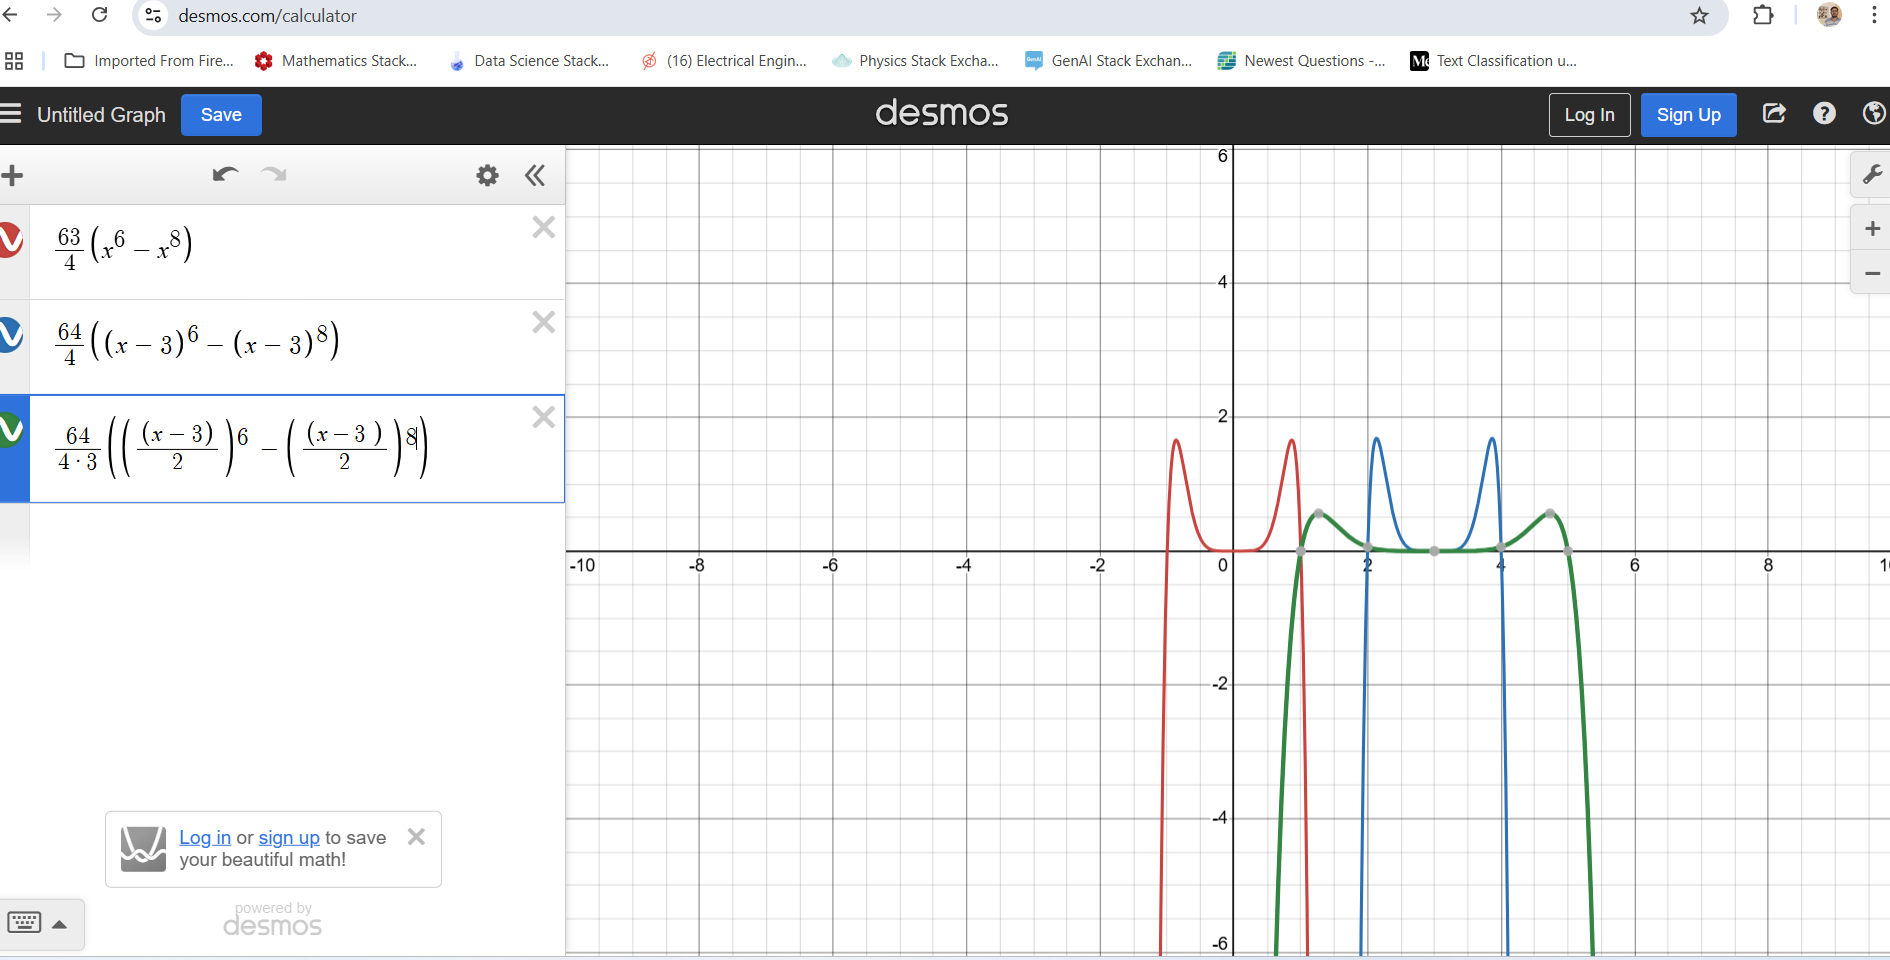
\includegraphics[width=0.7\linewidth]{screenshot001}
	\caption{}
	\label{fig:screenshot001}
\end{figure}
\newline
\section{}
$\left(\int_{-\infty}^{m}(\frac{1}{\sigma})f(\frac{x - \mu}{\sigma})dx\right) = \left(\int_{m}^{\infty}(\frac{1}{\sigma})f(\frac{x - \mu}{\sigma})dx\right)$
\newline
t = $\frac{x - \mu}{\sigma}$
substituting and differentiating
\newline
$\sigma$dt = dx
\newline
$\left(\int_{-\infty}^{\frac{m-\mu}{\sigma}}f(t)dt\right) = \frac{1}{2}$
\newline
$\frac{m - \mu}{\sigma} = 0$ $\Rightarrow$ m = $\mu$
\newline

\section{}
$(\frac{1}{\sigma})f(\frac{x - \mu}{\sigma})$
\newline
$x_{\alpha} = \sigma z_{\alpha} + \mu$
\newline
$\alpha = P(Z > z_\alpha) = \int_{z_\alpha}^{\infty}f(z)dz$
\newline
$z_{\alpha} = \frac{x_{\alpha} - \mu}{\sigma}$
$\alpha$ = $\int_{z_{\alpha}}^{\infty}f(z)dz$
\newline
Generalizing it $z = \frac{x - \mu}{\sigma}$
$\int_{\frac{x - \mu}{\sigma}}^{\infty}(\frac{1}{\sigma})f(\frac{x - \mu}{\sigma})dx = P(\frac{X - \mu}{\sigma} > \frac{x_{\alpha} - \mu}{\sigma}) = P(X > x_{\alpha}) = \alpha$
\newline

\section{}
(a) $\int_{-\infty}^{\mu}\frac{1}{\sigma \pi (1 + (\frac{x - \mu}{\sigma}))}dx = \int_{\mu}^{\infty}\frac{1}{\sigma \pi (1 + (\frac{x - \mu}{\sigma}))}dx$
substituting z = $\frac{x - \mu}{\sigma}$
\newline
we will get standard Cauchy with median 0. So x = $\mu$
\newline
(b) $\int_{-1}^{1}\frac{dx}{\sigma \pi \left(1 + \left(\frac{x - \mu}{\sigma}\right)^2\right)}$, putting $\mu$ = 0, $\sigma$ = 1.
We get $\frac{1}{2}$ With symmetry we get $\frac{1}{4}$  adding a general location ($\mu$) and scale family ($\sigma$)
\newline

\section{}
$f^*(x) = \frac{1}{\sigma}f(\frac{x - \mu}{\sigma})$
\newline

\section{}
Scholastically greater $F_X(t) \le F_Y(t)$ for all t
\newline
Say let X, Y = ${X + \mu'} \text{ } \text{are two random variables for same family distribution}$ where $\mu$' is fixed differences between the their mean.
P(t $\ge$ x) > P(t $\ge$ y) as for same $\sigma$ the area  as the distribution is same P(X) will be more than P(Y)
$F_X(x) > F_Y(y)$
\newline
Y is scholastically greater than X also Y is greater than X hence Provved
\newline
(b) Refer next section
\newline

\section{}
(a) For location family $\mu$ changes keeping the scale parameter constant, Refer to above section a logic you will get for the same.
\newline
(b) Let $\sigma_1 > \sigma_2$
\newline
$F(x|\sigma_1) = P(X_1 \le x) = P(\sigma_1Z \le x) = P(Z \le x\sigma_1) = F(x/\sigma_1) \le F(x/\sigma_2) = P(Z \le x/\sigma_2) = P(\sigma_2Z \le x) = P(X_2 \le x) = F(x | \sigma_2).$
\newline

\section{}
(a) $P( X \le x | \theta_1) \le P( X \le x | \theta_2)$
\newline
$\Rightarrow$ $P( \frac{1}{Y} \le \frac{1}{y} | \theta_1) \le P( \frac{1}{Y} \le \frac{1}{y} | \theta_2)$
\newline
$\Rightarrow$ $P( y \le Y | \theta_1) \le P( y \le Y | \theta_2)$
\newline
$\Rightarrow$ $P( Y \le y | \theta_1) \ge P( Y \le y | \theta_2)$
\newline
(b) P(X $\le$ x | $\theta$) $\le$ P(X $\le$ x | $\theta$ + $d\theta$)
\newline
P(X $le$ x | $\frac{1}{\theta}$), P(X $\le$ x | $\frac{1}{\theta}$ - $\frac{d\theta}{\theta^2}$)
\newline
Clearly P(X $le$ x | $\frac{1}{\theta}$)$\ge$ P(X $\le$ x | $\frac{1}{\theta}$ - $\frac{d\theta}{\theta^2}$)
\newline

\section{}
Using Chebychev Inequality's \newline
P(|X| $\ge$ b) $\le$ $\frac{E|X|}{b}$
\newline
P(|X| $\ge$ b) = P($X^{2}$ $\ge$ b) $\le$ $\frac{EX^2}{b^2}$
\newline
E|X|/b = 1/3 > 2/9 = $EX^2/b^2$
\newline
E|X|/b = 1/ $\sqrt{2}$ < 1 = $EX^2/b^2$.
\newline

\section{}
(a) $M_X(t) = \int_{-\infty}^{\infty}e^{tx}f_X(x)dx \text{ } \ge \text{ } \newline \int_{a}^{\infty}e^{tx}f_X(x)dx \text{ } \ge e^{ta} \int_{a}^{\infty}f_X(x)dx = e^{ta}P(X \ge a)$
\newline
(b) same as above
\newline
(c) It must be a non negative
\newline

\section{}
Draw graph
\newline

\section{}
(a) P(Z $\ge$ t) $\le$ $\int_{t}^{\infty}\frac{x^2 + 1}{x^2 + 1}e^{-\frac{x^2}{2}}dx = \int_{t}^{\infty}\frac{x^2}{x^2 + 1}e^{-\frac{x^2}{2}}dx + \int_{t}^{\infty}\frac{1}{x^2 + 1}e^{-\frac{x^2}{2}}dx$
\newline
On solving first you will get the equality. Second term must be discarded
\newline

\section{}
(a),(b),(c) Divide P(X = x+1)/P(X = x) to derive it for all
\newline

\section{}
(a)(b) solve mathematically
\newline

\section{}
(a)(b) solve mathematically
\newline


		
\end{document}